\documentclass{article}
%\usepackage{figure}
\usepackage{graphicx}
\usepackage{float}
\usepackage{setspace}

\usepackage[a4paper, left=.6in, right=.6in, top=1in, bottom=1.2in]{geometry}
\begin{document}
\doublespacing
\begin{itemize}
    \item$\xi_p= 1000$:
        \begin{figure}[H]
            \centering
            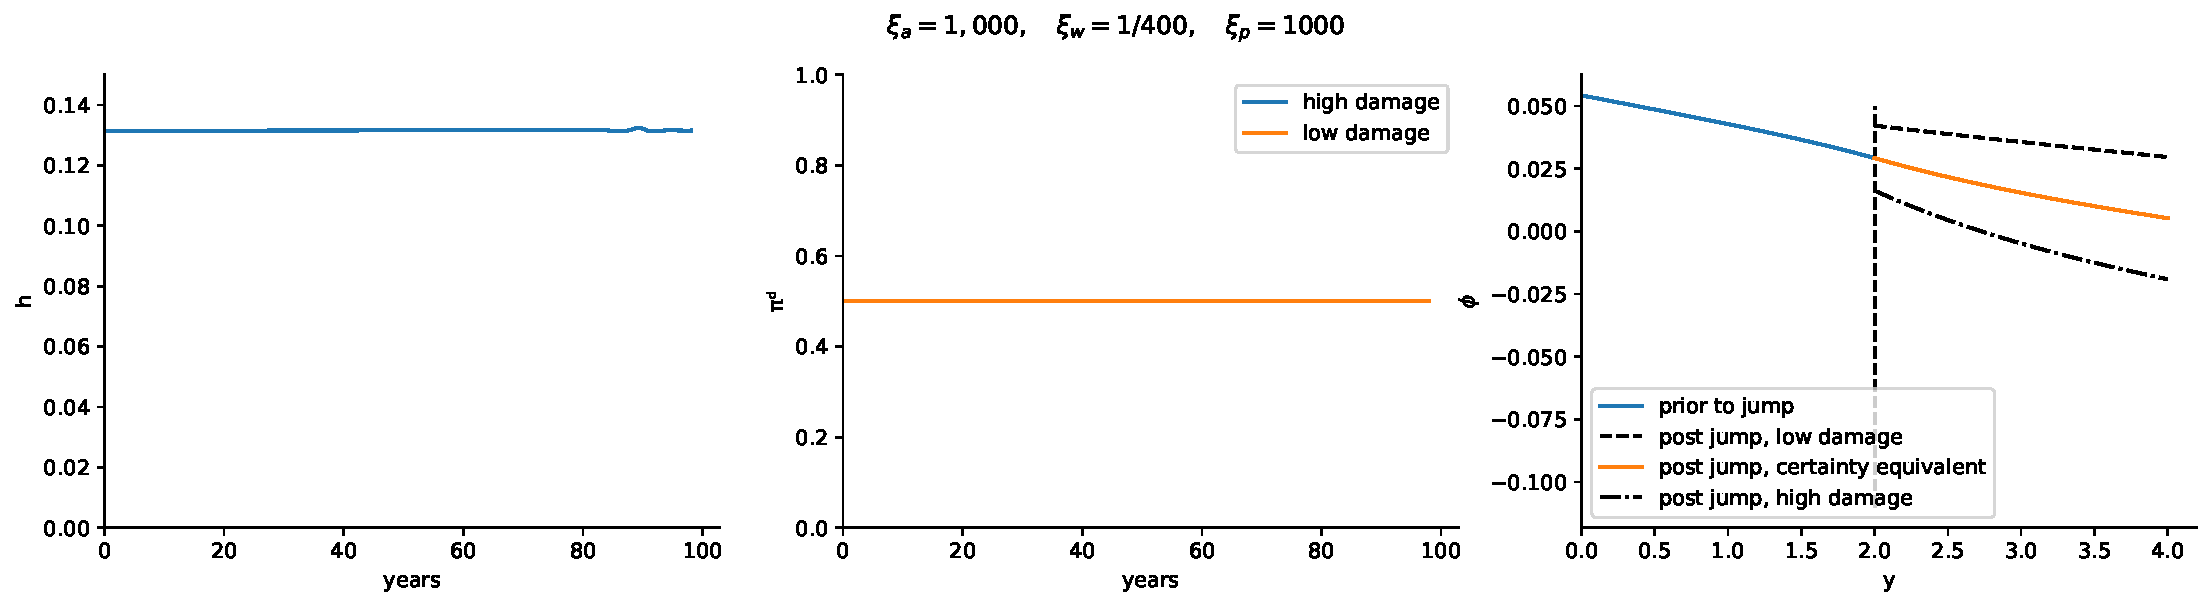
\includegraphics[width=\linewidth]{notebook/phi_n.pdf}
            \caption{$\xi_p=1000$,  $h$(left), $\pi_i^p$ (center) and $\phi(y)$ (right)}
            \label{fig:notebook/phi_n}
        \end{figure}
\item $\xi_p=10\xi_w$
    \begin{figure}[H]
        \centering
        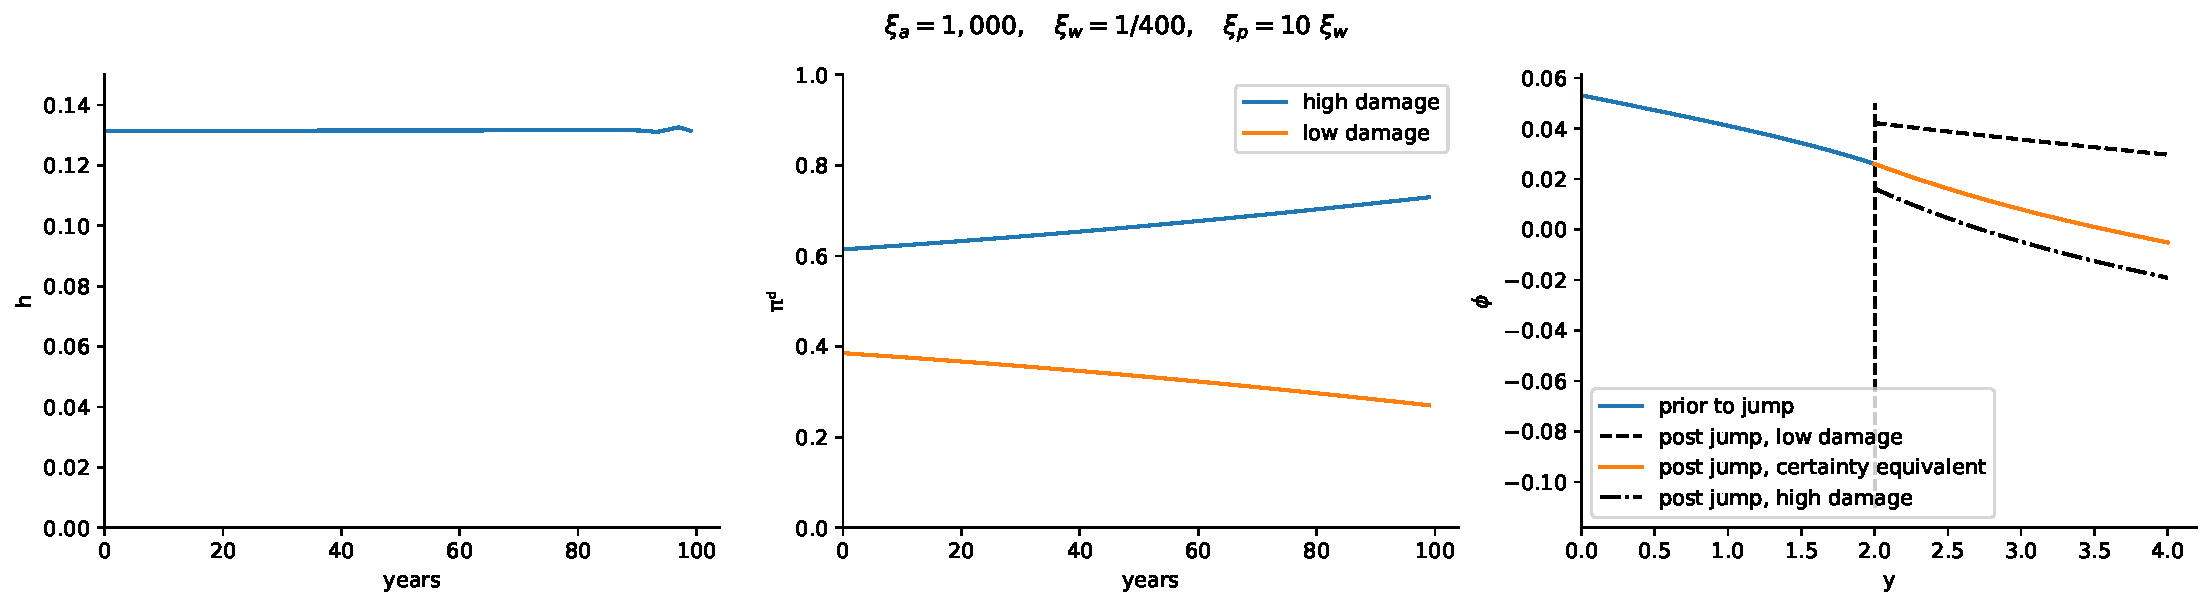
\includegraphics[width=\linewidth]{notebook/phi_x10.pdf}
        \caption{$\xi_p= 10\xi_w$, $h$(left), $\pi_i^p$ (center) and $\phi(y)$ (right)}
        \label{fig:notebook/phi_x10}
    \end{figure}
\item$\xi_p= 5\xi_w$:
       \begin{figure}[H]
           \centering
           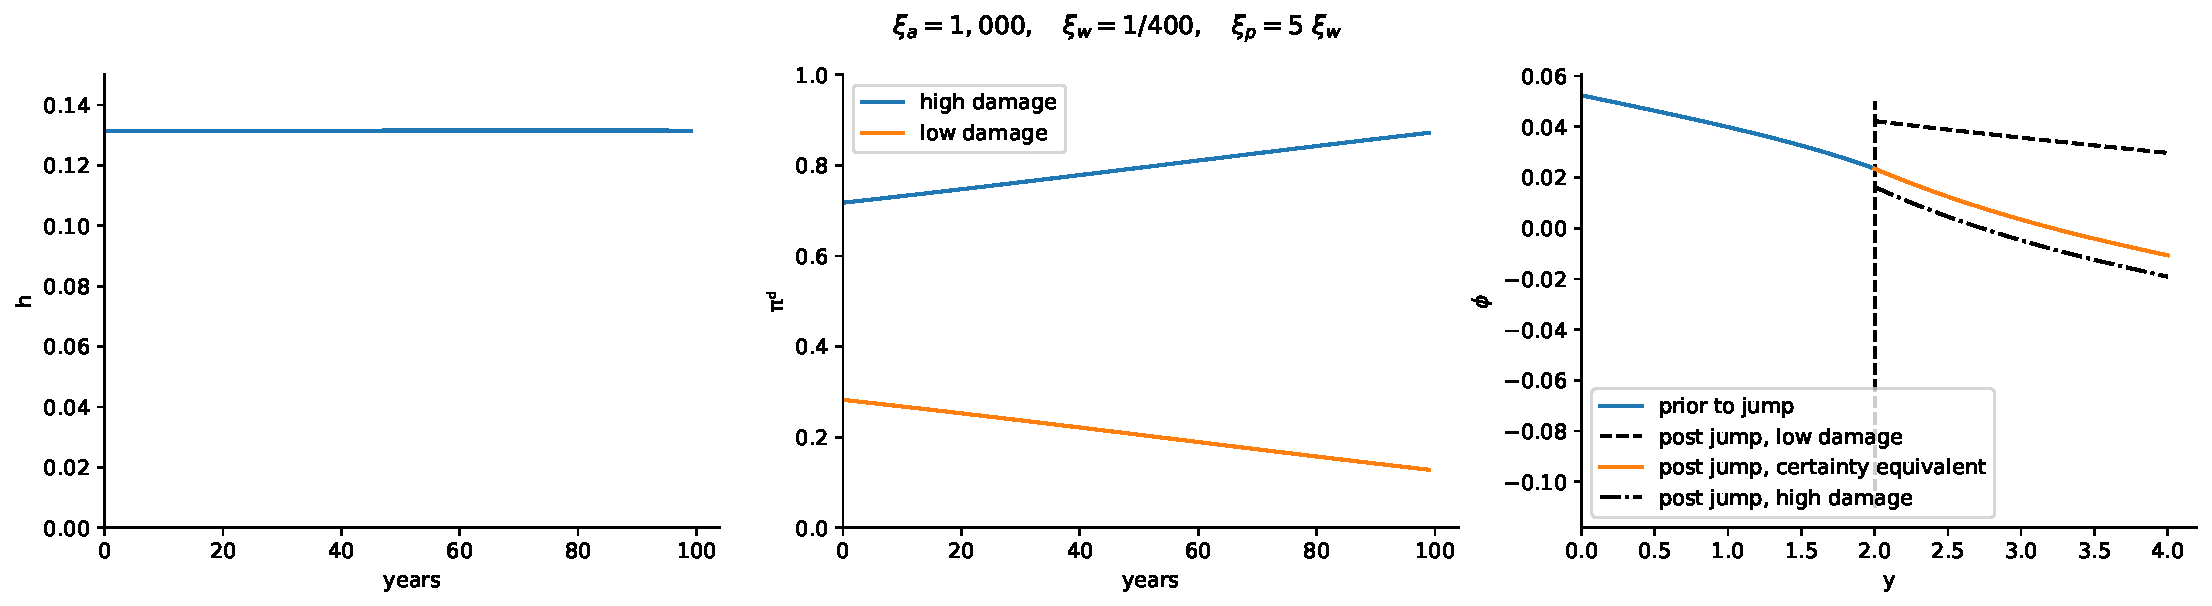
\includegraphics[width=\linewidth]{notebook/phi_x5.pdf}
           \caption{$\xi_p= 5\xi_w$, $h$(left), $\pi_i^p$ (center) and $\phi(y)$ (right)}
           \label{fig:notebook/phi_x5}
       \end{figure}
       \newpage
    \item$\xi_p=\xi_w$
\begin{figure}[H]
    \centering
    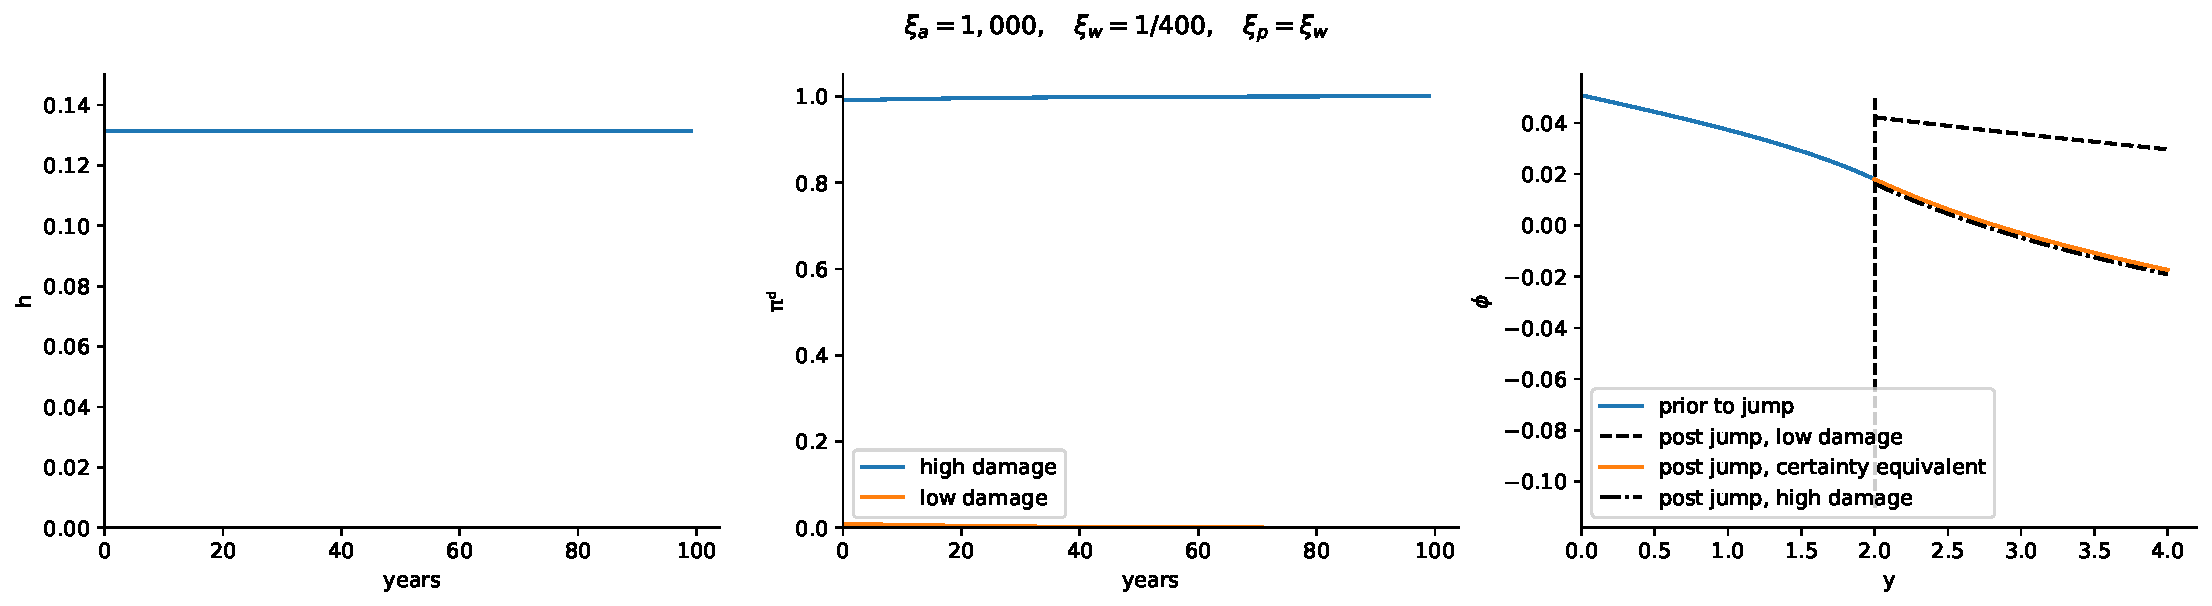
\includegraphics[width=\linewidth]{notebook/phi_x1.pdf}
    \caption{$\xi_p=\xi_w$, $h$(left), $\pi_i^p$ (center) and $\phi(y)$ (right)}
    \label{fig:notebook/phi_x1}
\end{figure}
\item$\tilde e$ and $SCC$:
    \begin{figure}[htpb]
        \centering
        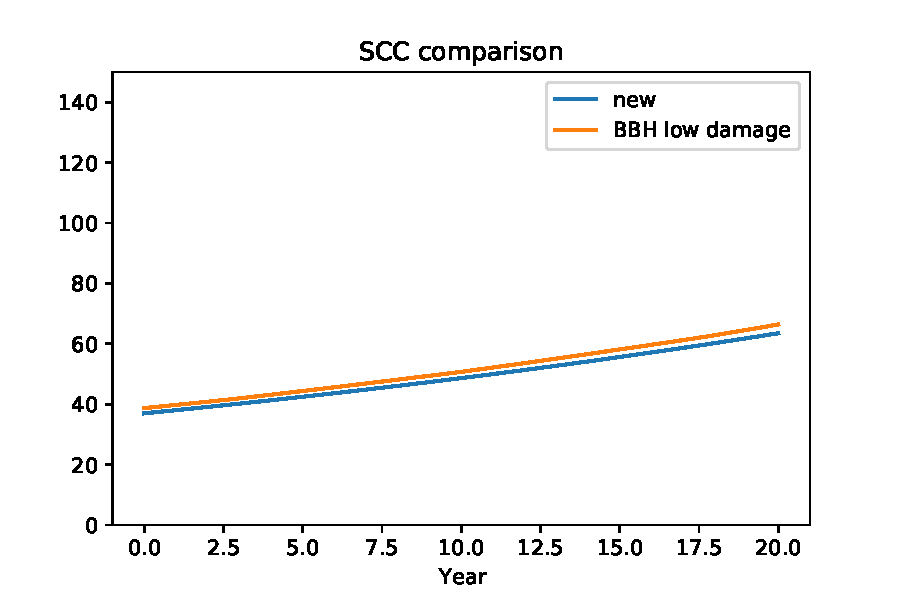
\includegraphics[width= \linewidth]{notebook/scc.pdf}
        \caption{$\tilde e$(left) and $SCC$(right)}
        \label{fig:notebook/scc}
    \end{figure}
\end{itemize}
\end{document}
